% Asal-usul (tidak pernah dicetak): lihat sources/outline_sources.md (Tahun 1: sirkulasi umum atmosfer, sel Hadley, Ferrel dan kutub, ITCZ, sel Walker, arus jet, angin geostrofik, depresi dan antisiklon). Nilai soal dan latihan dari kalkulator skrip Buku 3 calc/ch28.py; gambar dari figdata/bachelor-1/angular_momentum_wind.py, weather_map.py (peta fiktif) dan general_circulation.py (NCEP-NCAR Reanalysis 1, rerata jangka panjang 1991-2020, dataset bachelor-1-ncep-{uwnd-p,vwnd-p,uwnd-sfc,slp,prate-monthly}).
% Fisika memiliki gaya Coriolis dan relasi hidrostatik (diingat kembali). Buku 1 (kelas 8) memberi angin global, sel konveksi, depresi dan antisiklon, isobar dan perputaran angin di sekelilingnya, dengan kata-kata: di sini dibangun ulang dengan gaya dan data. ENSO dan monsun adalah volume Tahun 2; angin termal adalah volume Tahun 3.
\chapter{Sirkulasi umum atmosfer}\label{ch:b1:atmospheric-circulation}

Kapal layar yang berlayar dari Eropa dan Afrika ke Amerika mengandalkan \omterm{def:b1:atmospheric-circulation:winds}{angin pasat}, angin timur yang tetap di tropik. Lebih dekat ke khatulistiwa, dalam sekitar lima derajat darinya, angin yang sama mereda, di sabuk keteduhan dan hujan deras yang bertahan, yang oleh para pelaut disebut doldrum. Jauh di atas keduanya, sekitar sembilan kilometer, sungai-sungai udara sempit yang disebut \omterm{def:b1:atmospheric-circulation:jet}{arus jet} dapat berhembus lebih dari \qty{440}{km/h}. Bab ini menjelaskan ketiganya: mengapa udara yang bergerak di atas planet yang berotasi berakhir berhembus sepanjang isobar, bukan melintasinya; bagaimana surplus tropik menggerakkan sel sirkulasi besar di kedua sisi khatulistiwa; dan mengapa udara yang meninggalkan khatulistiwa di ketinggian berubah menjadi \omterm{def:b1:atmospheric-circulation:jet}{arus jet} barat.
% ledger: nos:trade-winds, nos:doldrums, noaajs:jet

\begin{omfigure}
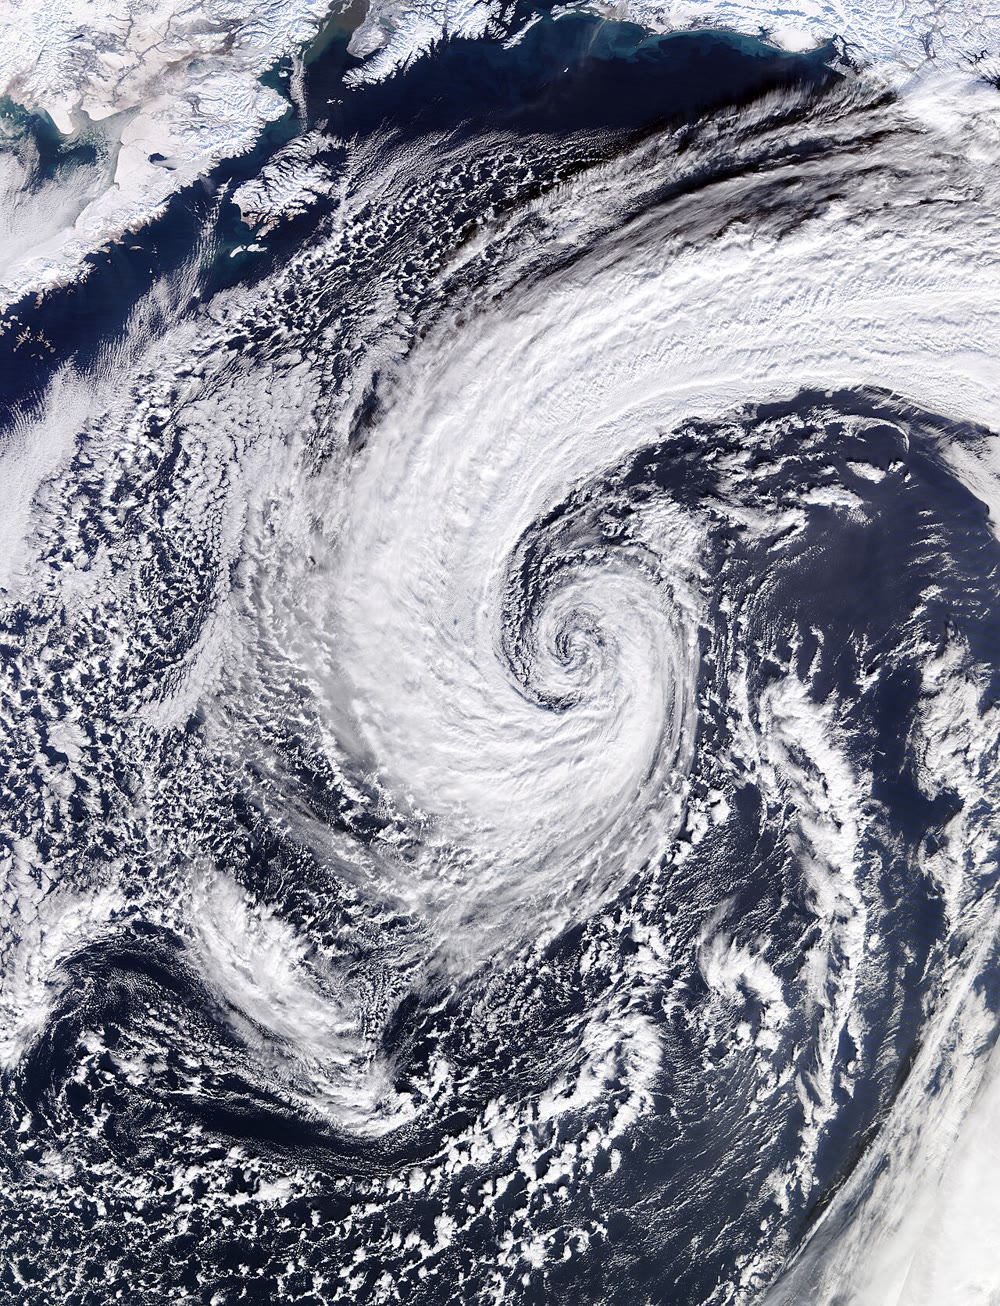
\includegraphics[width=0.5\linewidth]{images/book3/b1-alaska-low.jpg}

{\small \omterm{def:b1:atmospheric-circulation:cyclone}{Siklon} ekstratropis di atas Teluk Alaska pada 28 Januari 2018, dilihat oleh instrumen MODIS dari orbit; pantai Alaska yang tertutup salju ada di kiri atas, dan utara kira-kira di atas. Pita-pita awan memutar berlawanan arah jarum jam menuju pusatnya, seperti yang dilakukan udara dalam depresi Belahan Utara. (NASA, MODIS/LANCE, domain publik, melalui Wikimedia Commons.)}
\label{fig:b1:atmospheric-circulation:alaska}
\end{omfigure}
% ledger: commons:alaska-low, nws:cyclone

\begin{recall}
Buku-buku fisika memberikan relasi hidrostatik dan gaya Coriolis: dalam kerangka yang berotasi dengan kecepatan sudut $\vec\Omega$, sebuah benda bermassa $m$ yang bergerak dengan kecepatan $\vec v$ relatif terhadap kerangka itu merasakan gaya semu $-2m\,\vec\Omega\times\vec v$, tegak lurus terhadap geraknya. Untuk Bumi, $\Omega = 2\pi/T_\star$ dengan hari sideris $T_\star = \qty{23.9345}{h}$, yaitu $\Omega = \qty{7.292e-5}{rad.s^{-1}}$. Buku~1 menjelaskan angin global (\omterm{def:b1:atmospheric-circulation:winds}{angin pasat}, \omterm{def:b1:atmospheric-circulation:winds}{angin barat}, angin timur kutub), sel konveksi, depresi dan \omterm{def:b1:atmospheric-circulation:cyclone}{antisiklon}, isobar pada peta cuaca, dan berbeloknya angin di sekitar pusatnya. \Cref{ch:b1:fluid-envelopes-structure} memberi \omterm{def:b1:fluid-envelopes-structure:standard-atmosphere}{atmosfer standar} dan laju lapse adiabatik kering, dan \cref{ch:b1:radiation-heat-transport} transpor panas ke arah kutub yang dibawa sirkulasi.
% ledger: earth:Trot, nws:coriolis
\end{recall}

\section{Gaya pada udara yang bergerak}\label{sec:b1:atmospheric-circulation:forces}

Sebuah \omterm{def:b1:fluid-envelopes-structure:parcel}{parsel udara} didorong oleh tekanan udara di sekitarnya, ditarik gravitasi, diperlambat oleh gesekan di dekat tanah, dan, dilihat dari Bumi yang berotasi, dibelokkan oleh gaya Coriolis. Gravitasi dan gaya tekan vertikal saling mengimbangi hampir sempurna: inilah relasi hidrostatik. Cuaca dibuat oleh gaya-gaya yang tersisa dalam arah horizontal.

\begin{definition}[Gaya gradien tekanan]\label{def:b1:atmospheric-circulation:pgf}
\emph{Gaya gradien tekanan}\index{gaya gradien tekanan} adalah gaya neto yang dikerjakan pada sebuah parsel fluida oleh tekanan fluida di sekitarnya. Per satuan massa ia adalah $-(1/\rho)\nabla p$, dengan $\rho$ massa jenis dan $\nabla p$ gradien tekanan: ia mengarah dari tekanan tinggi ke tekanan rendah, melintasi isobar.
\end{definition}
% ledger: nws:geostrophic

\begin{proposition}[Gaya gradien tekanan]\label{prop:b1:atmospheric-circulation:pgf}
Pada sebuah parsel bervolume $\mathrm dV$ dan massa jenis $\rho$, tekanan fluida di sekitarnya mengerjakan gaya $-\nabla p\,\mathrm dV$, yaitu percepatan $-(1/\rho)\nabla p$.
\end{proposition}

\begin{proof}
Ambil kotak kecil dengan sisi $\mathrm dx$, $\mathrm dy$, $\mathrm dz$ sepanjang sumbu-sumbu.
Pada sisi di $x$, tekanan mendorong ke arah $+x$ dengan gaya
$p(x)\,\mathrm dy\,\mathrm dz$; pada sisi di $x + \mathrm dx$, ke arah $-x$ dengan
$p(x + \mathrm dx)\,\mathrm dy\,\mathrm dz$. Gaya neto sepanjang
$x$ adalah $[p(x) - p(x + \mathrm dx)]\,\mathrm dy\,\mathrm dz = -(\partial p/\partial
x)\,\mathrm dV$, dan demikian pula sepanjang $y$ dan $z$. Totalnya adalah $-\nabla p\,
\mathrm dV$; membaginya dengan massa $\rho\,\mathrm dV$ memberi percepatan.
\end{proof}

Tekanan yang seragam tidak mengerjakan gaya neto: hanya selisihnya yang mendorong. Pada peta cuaca, gradien horizontal dibaca dari isobar: besarnya adalah lompatan tekanan antara dua isobar dibagi jaraknya. Untuk isobar yang berjarak \qty{4}{hPa} dan \qty{400}{km} di permukaan laut, tempat $\rho \approx \qty{1.225}{kg.m^{-3}}$, percepatannya adalah $400/(1.225 \times \num{4e5}) = \qty{8.2e-4}{m.s^{-2}}$, kurang dari sepersepuluh ribu $g$, namun cukup untuk membawa udara dari diam hingga \qty{10}{m/s} dalam tiga setengah jam.
% ledger: ussa76:sea-level

Udara merasakan gaya Coriolis karena ia diamati dari Bumi yang berputar. Bagian horizontalnya bergantung pada \omterm{def:b1:spherical-astronomy:geographic}{lintang} melalui satu bilangan tunggal.

\begin{definition}[Parameter Coriolis]\label{def:b1:atmospheric-circulation:coriolis-parameter}
\emph{Parameter Coriolis}\index{parameter Coriolis} pada \omterm{def:b1:spherical-astronomy:geographic}{lintang} $\varphi$ adalah $f = 2\Omega\sin\varphi$, dengan $\Omega$ kecepatan sudut Bumi. Ia positif di Belahan Utara, negatif di Selatan, nol di khatulistiwa, dan terbesar di kutub, $2\Omega = \qty{1.458e-4}{s^{-1}}$.
\end{definition}
% ledger: earth:Trot

\begin{proposition}[Percepatan Coriolis horizontal]\label{prop:b1:atmospheric-circulation:coriolis}
Untuk angin horizontal $\vec v$ pada \omterm{def:b1:spherical-astronomy:geographic}{lintang} $\varphi$, bagian horizontal percepatan Coriolis adalah $-f\,\vec k\times\vec v$, dengan $\vec k$ vertikal ke atas: ia memiliki besar $|f|\,|\vec v|$ dan mengarah tegak lurus terhadap angin, ke kanannya di Belahan Utara dan ke kirinya di Selatan.
\end{proposition}

\begin{proof}
Gunakan sumbu lokal $x$ ke timur, $y$ ke utara, $z$ ke atas. Vektor rotasi Bumi berada pada bidang meridian,
dengan sudut $\varphi$ di atas cakrawala utara: $\vec\Omega =
\Omega(0, \cos\varphi, \sin\varphi)$. Untuk $\vec v = (u, v, 0)$,
\[
  \vec\Omega\times\vec v = \Omega\,(-v\sin\varphi,\ u\sin\varphi,\ -u\cos\varphi),
  \qquad -2\vec\Omega\times\vec v = (f v,\ -f u,\ 2\Omega u\cos\varphi).
\]
Karena $\vec k\times\vec v = (-v, u, 0)$, bagian horizontal $(fv, -fu)$ adalah
$-f\,\vec k\times\vec v$. Vektor $\vec k\times\vec v$ adalah $\vec v$ yang diputar sebesar
\ang{90} berlawanan arah jarum jam jika dilihat dari atas; kebalikannya adalah $\vec v$ yang diputar searah jarum jam,
ke kanan, bila $f > 0$, dan ke kiri bila $f < 0$.
\end{proof}
% ledger: earth:Trot

Bagian vertikal, $2\Omega u\cos\varphi$, paling besar \qty{1.5e-3}{m.s^{-2}} untuk angin \qty{10}{m/s}, sekitar \num{1.5e-4} dari $g$: keseimbangan hidrostatik menyerapnya. Bagian horizontal, meski kecil, tidak memiliki saingan di atmosfer bebas di atas lapisan gesekan, dan dalam hitungan jam ia membentuk setiap angin.

Dekat tanah, udara juga bergesekan dengan permukaan. Di kilometer terbawah, lapisan gesekan para meteorolog, gesekan mengubah baik kelajuan maupun arah angin; pusaran turbulen membawa seret permukaan ke atas, dan gaya itu bekerja kurang lebih melawan angin dan bertambah dengan kelajuannya. Di atas, di atmosfer bebas, gesekan kecil.
% ledger: nws:friction-layer

\section{Angin geostrofik}\label{sec:b1:atmospheric-circulation:geostrophic}

\begin{definition}[Keseimbangan geostrofik, angin geostrofik]\label{def:b1:atmospheric-circulation:geostrophic}
Aliran horizontal berada dalam \emph{keseimbangan geostrofik}\index{keseimbangan geostrofik} bila \omterm{def:b1:atmospheric-circulation:pgf}{gaya gradien tekanannya} dan gaya Coriolisnya saling meniadakan. \emph{Angin geostrofik}\index{angin geostrofik} $\vec v_g$ adalah angin yang mencapai keseimbangan ini untuk medan tekanan tertentu: $-(1/\rho)\nabla p - f\,\vec k\times\vec v_g = \vec 0$.
\end{definition}
% ledger: nws:geostrophic

\begin{theorem}[Angin geostrofik]\label{thm:b1:atmospheric-circulation:geostrophic}
Jauh dari khatulistiwa,
\[
  \vec v_g = \frac{1}{\rho f}\,\vec k\times\nabla p, \qquad
  |\vec v_g| = \frac{|\nabla p|}{\rho\,|f|} .
\]
\omterm{def:b1:atmospheric-circulation:geostrophic}{Angin geostrofik} berhembus sepanjang isobar, lebih cepat di tempat isobar makin rapat. Di Belahan Utara ia menjaga tekanan rendah di sebelah kirinya; di Belahan Selatan, di sebelah kanannya.
\end{theorem}

\begin{proof}
Untuk vektor horizontal $\vec w$, $\vec k\times(\vec k\times\vec w) = -\vec w$.
Menerapkan $\vec k\times$ pada keseimbangan $f\,\vec k\times\vec v_g = -(1/\rho)\nabla p$
memberi $-f\vec v_g = -(1/\rho)\,\vec k\times\nabla p$, sehingga rumusnya, berlaku bila
$f \neq 0$. Karena $\vec k\times\nabla p$ tegak lurus terhadap $\nabla p$, angin tegak lurus
terhadap gradien, yaitu sepanjang isobar; besarnya adalah $|\nabla
p|/(\rho|f|)$. Vektor $\vec k\times\nabla p$ adalah gradien yang diputar \ang{90}
berlawanan arah jarum jam. Dengan menghadap ke arahnya, gradien, yang menunjuk ke tekanan tinggi,
berada di sebelah kanan, sehingga tekanan rendah berada di sebelah kiri; untuk $f > 0$ angin memiliki
arah $\vec k\times\nabla p$, untuk $f < 0$ arah sebaliknya.
\end{proof}

\begin{example}[Angin dibaca dari isobar]\label{ex:b1:atmospheric-circulation:geostrophic}
Pada \ang{50} LU, $f = 2 \times \num{7.292e-5} \times \sin\ang{50} = \qty{1.117e-4}{s^{-1}}$.
Isobar yang berjarak \qty{4}{hPa} dan \qty{400}{km} memberi $|\nabla p| = 400/\num{4e5} =
\qty{1.0e-3}{Pa.m^{-1}}$ dan, dengan $\rho = \qty{1.225}{kg.m^{-3}}$, \omterm{def:b1:atmospheric-circulation:geostrophic}{angin geostrofik}
sebesar $\num{1.0e-3}/(1.225 \times \num{1.117e-4}) = \qty{7.3}{m/s}$. Jarak yang sama
pada \ang{20} LU, tempat $f$ kurang dari setengahnya, akan memberi
\qty{16.4}{m/s}.
\end{example}
% ledger: earth:Trot, ussa76:sea-level

Keseimbangan itu tidak seketika. Udara yang digerakkan oleh gradien tekanan berbelok di bawah gaya Coriolis dengan laju $f$, kira-kira sekali setiap $2\pi/f$, sekitar enam belas jam pada \ang{50}; pola yang bertahan lebih lama dari beberapa jam, dan lebih besar dari beberapa ratus kilometer, mendekati geostrofik. Dekat khatulistiwa $f$ cenderung nol, rumusnya gagal, dan angin di tropik dalam tidak geostrofik.

\begin{omfigure}
\begin{tikzpicture}[>={Stealth[length=2.2mm]}, font=\scriptsize]
  % left panel: geostrophic balance
  \begin{scope}
    \draw[isobar] (-2.4,1.2) -- (2.4,1.2) node[right] {\qty{996}{hPa}};
    \draw[isobar] (-2.4,0) -- (2.4,0) node[right] {\qty{1000}{hPa}};
    \draw[isobar] (-2.4,-1.2) -- (2.4,-1.2) node[right] {\qty{1004}{hPa}};
    \node[pressure low] at (0,2.0) {L};
    \node[pressure high] at (0,-2.0) {H};
    \fill (0,0) circle (1.6pt);
    \draw[->, very thick, omThm] (0,0) -- (0,1.0);
    \node[omThm, anchor=east] at (-0.08,0.6) {gradien tekanan};
    \draw[->, very thick, omDef] (0,0) -- (0,-1.0);
    \node[omDef, anchor=east] at (-0.08,-0.6) {Coriolis};
    \draw[->, line width=1.6pt, black] (0,0) -- (1.9,0) node[above, pos=0.75] {angin $\vec v_g$};
    \node[anchor=north] at (0,-2.4) {tanpa gesekan: geostrofik};
  \end{scope}
  % right panel: with friction (alpha = 25 deg, V = Vg cos alpha)
  \begin{scope}[xshift=7.4cm]
    \draw[isobar] (-2.4,1.2) -- (2.4,1.2) node[right] {\qty{996}{hPa}};
    \draw[isobar] (-2.4,0) -- (2.4,0) node[right] {\qty{1000}{hPa}};
    \draw[isobar] (-2.4,-1.2) -- (2.4,-1.2) node[right] {\qty{1004}{hPa}};
    \node[pressure low] at (0,2.0) {L};
    \node[pressure high] at (0,-2.0) {H};
    \fill (0,0) circle (1.6pt);
    \draw[->, very thick, omThm] (0,0) -- (0,1.0);
    \node[omThm, anchor=east] at (-0.08,0.6) {gradien tekanan};
    \draw[->, very thick, omDef] (0,0) -- ({1.0*cos(25)*sin(25)},{-1.0*cos(25)*cos(25)});
    \node[omDef, anchor=west] at (0.42,-0.62) {Coriolis};
    \draw[->, very thick, omMeth] (0,0) -- ({-1.0*sin(25)*cos(25)},{-1.0*sin(25)*sin(25)})
      node[below left, inner sep=1pt] {gesekan};
    \draw[->, line width=1.6pt, black] (0,0) -- ({1.9*cos(25)*cos(25)},{1.9*cos(25)*sin(25)})
      node[above, inner sep=2pt] {angin $\vec v$};
    \draw[black!50, dashed] (0,0) -- (1.9,0);
    \draw[black!60] (1.0,0) arc[start angle=0, end angle=25, radius=1.0];
    \node[black!70] at (1.22,0.22) {$\alpha$};
    \node[anchor=north] at (0,-2.4) {dengan gesekan: lebih lambat, melintasi isobar};
  \end{scope}
\end{tikzpicture}

{\small Gaya pada sebuah \omterm{def:b1:fluid-envelopes-structure:parcel}{parsel udara} di Belahan Utara, dengan tekanan rendah di utara. Kiri: di atmosfer bebas \omterm{def:b1:atmospheric-circulation:pgf}{gaya gradien tekanan} (merah) dan gaya Coriolis (biru) saling meniadakan, dan angin berhembus sepanjang isobar dengan rendah di sebelah kirinya. Kanan: dekat tanah gesekan (hijau) bekerja melawan angin; ketiga gaya itu seimbang hanya bila angin lebih lambat dan berbelok sebesar sudut $\alpha$ ke arah rendah (digambar untuk $\alpha = \ang{25}$ dan seret dari \cref{prop:b1:atmospheric-circulation:friction}).}
\label{fig:b1:atmospheric-circulation:balance}
\end{omfigure}

\begin{proposition}[Gesekan membelokkan angin ke arah tekanan rendah]\label{prop:b1:atmospheric-circulation:friction}
Misalkan angin horizontal mantap $\vec v$ dikenai \omterm{def:b1:atmospheric-circulation:pgf}{gaya gradien tekanan},
gaya Coriolis dan gaya gesekan $-\vec v/\tau$, dengan $\tau > 0$, pada \omterm{def:b1:spherical-astronomy:geographic}{lintang}
dengan $f > 0$. Maka angin melintasi isobar menuju tekanan rendah pada sudut $\alpha$
dengan $\tan\alpha = 1/(f\tau)$, dan kelajuannya $|\vec v| =
|\vec v_g|\cos\alpha$, lebih kecil daripada \omterm{def:b1:atmospheric-circulation:geostrophic}{angin geostrofik}.
\end{proposition}

\begin{proof}
Misalkan $V = |\vec v|$, $\hat v$ vektor satuan sepanjang angin dan $\hat n$ vektor
satuan yang tegak lurus terhadapnya, di sebelah kirinya. Keseimbangannya adalah $-(1/\rho)\nabla p - f\,
\vec k\times\vec v - \vec v/\tau = \vec 0$, dan $\vec k\times\vec v = V\hat n$.
Sepanjang $\hat v$: $-(1/\rho)\,\nabla p\cdot\hat v = V/\tau > 0$, sehingga angin memiliki
komponen menuruni gradien tekanan, menuju tekanan rendah. Sepanjang $\hat n$:
$-(1/\rho)\,\nabla p\cdot\hat n = fV$. \omterm{def:b1:atmospheric-circulation:pgf}{Gaya gradien tekanan}, berbesar $P =
|\nabla p|/\rho = f|\vec v_g|$, karena itu memiliki komponen $V/\tau$ sepanjang angin dan
$fV$ melintasinya: ia membentuk dengan angin sudut $\beta$ dengan $\tan\beta =
1/(f\tau)$, dan $P^2 = V^2(f^2 + 1/\tau^2)$. Isobar tegak lurus terhadap gradien, sehingga angin
melintasinya pada $\alpha = \beta$, dan $V = P/\sqrt{f^2 +
1/\tau^2} = (P/f)\cos\alpha = |\vec v_g|\cos\alpha$.
\end{proof}

Permukaan yang lebih kasar berarti seret yang lebih kuat, $\tau$ yang lebih pendek dan sudut yang lebih besar: angin melintasi isobar dengan lebih curam di atas daratan daripada di atas laut. Gesekan sungguhan tidak tepat linear terhadap angin, tetapi kesimpulannya, lebih lambat dan berbelok ke arah rendah, bersifat umum.

\begin{remark}[Angin gradien]\label{rem:b1:atmospheric-circulation:gradient}
Di sekitar pusat, isobar melengkung, dan udara yang mengikutinya dipercepat menuju pusat kelengkungan, sebesar $V^2/r$ untuk lingkaran berjari-jari $r$. Di sekitar rendah di Belahan Utara, \omterm{def:b1:atmospheric-circulation:pgf}{gaya gradien tekanan} harus melebihi gaya Coriolis: $fV + V^2/r = f|\vec v_g|$, dan angin, yang disebut angin gradien, lebih lemah daripada \omterm{def:b1:atmospheric-circulation:geostrophic}{angin geostrofik}. Di sekitar tinggi, gaya Coriolis harus melebihi \omterm{def:b1:atmospheric-circulation:pgf}{gaya gradien tekanan}, $fV - V^2/r = f|\vec v_g|$: anginnya lebih kuat, tetapi persamaannya memiliki solusi hanya bila $|\vec v_g| \leq fr/4$, yang melarang gradien tekanan kuat di dekat pusat \omterm{def:b1:atmospheric-circulation:cyclone}{antisiklon} (\cref{exo:b1:atmospheric-circulation:10}).
\end{remark}

\section{Depresi dan antisiklon}\label{sec:b1:atmospheric-circulation:cyclones}

\begin{definition}[Siklon, antisiklon]\label{def:b1:atmospheric-circulation:cyclone}
Sebuah \emph{siklon}\index{siklon} adalah sirkulasi skala besar angin di sekitar pusat tekanan rendah, yaitu depresi; \emph{antisiklon}\index{antisiklon} adalah sirkulasi di sekitar pusat tekanan tinggi. Siklon berputar berlawanan arah jarum jam di Belahan Utara dan searah jarum jam di Selatan; antisiklon sebaliknya.
\end{definition}
% ledger: nws:cyclone

Arah putaran ini diperoleh dari \cref{thm:b1:atmospheric-circulation:geostrophic}: di Belahan Utara, angin yang menjaga tekanan rendah di sebelah kirinya berputar mengelilingi rendah berlawanan arah jarum jam dan mengelilingi tinggi searah jarum jam. Dilihat dari angkasa, awan depresi menelusuri putarannya (foto di awal bab); di Belahan Selatan spiralnya merupakan bayangan cermin.
% ledger: nws:cyclone, commons:alaska-low

\begin{history}[Hukum Buys Ballot, 1857]
Pada 1857 meteorolog Belanda C.~H.~D. Buys Ballot menyatakan suatu aturan yang ditemukan dalam observasi: di Belahan Utara, seseorang yang berdiri membelakangi angin memiliki tekanan rendah di sebelah kiri dan tekanan tinggi di sebelah kanan; di Belahan Selatan, sebaliknya. Ia tidak tahu bahwa meteorolog Amerika William Ferrel telah menurunkannya dari teori, dan kemudian mengakui prioritas Ferrel. \omterm{def:b1:atmospheric-circulation:geostrophic}{Angin geostrofik} adalah hukum itu dalam persamaan.
\end{history}
% ledger: skybrary:buys-ballot

Gesekan menambahkan puntiran penting. Dekat tanah angin melintasi isobar menuju tekanan rendah (\cref{prop:b1:atmospheric-circulation:friction}): di sekitar depresi udara berspiral ke dalam, berkonvergensi dekat tanah, dan harus naik. Udara yang naik memuai dan mendingin dengan laju lapse adiabatik kering (\cref{ch:b1:fluid-envelopes-structure}), dan begitu jenuh uap airnya mengembun: depresi membawa awan dan hujan. Di sekitar \omterm{def:b1:atmospheric-circulation:cyclone}{antisiklon} udara permukaan berspiral ke luar; udara turun dari atas untuk menggantikannya, menghangat karena kompresi, dan awannya menguap: \omterm{def:b1:atmospheric-circulation:cyclone}{antisiklon} membawa cuaca yang mantap, sering cerah.
% ledger: nws:dalr

Peta di bawah adalah contoh fiktif, dihitung bukan diamati: sebuah depresi \qty{28}{hPa} dalam dan sebuah \omterm{def:b1:atmospheric-circulation:cyclone}{antisiklon} \qty{20}{hPa} tinggi pada latar \qty{1013}{hPa}, berpusat dekat \ang{50} LU. Di setiap stasiun, panah angin menunjukkan \omterm{def:b1:atmospheric-circulation:geostrophic}{angin geostrofik} yang dihitung dari peta dengan \cref{thm:b1:atmospheric-circulation:geostrophic}.

\begin{omfigure}
\pgfplotstableread{figdata/out/bachelor-1-weather_map-stations.dat}\wmstations
\pgfplotstableread{figdata/out/bachelor-1-weather_map-labels.dat}\wmlabels
\begin{tikzpicture}
\begin{axis}[x=0.0038cm, y=0.0038cm, disabledatascaling, anchor=origin,
  xmin=-1800, xmax=1800, ymin=-1200, ymax=1200, xtick=\empty, ytick=\empty,
  axis background/.style={fill=blue!4}, clip=true]
% figdata/bachelor-1/weather_map.py (invented pressure field); ledger: earth:Trot, ussa76:sea-level
\addplot[isobar, unbounded coords=jump] table[x=x, y=y] {figdata/out/bachelor-1-weather_map-isobars.dat};
\addplot[black!45, dashed, domain=-1800:1800] {0};
\addplot[only marks, mark=none, nodes near coords, point meta=explicit symbolic,
  nodes near coords style={font=\tiny, fill=blue!4, inner sep=0.5pt, anchor=center}]
  table[x=x, y=y, meta=p] {\wmlabels};
\node[pressure low] at (axis cs:-500,150) {L};
\node[pressure high] at (axis cs:1050,-250) {H};
\node[font=\tiny, anchor=south west, black!60] at (axis cs:-1790,5) {\ang{50} LU};
\end{axis}
\pgfplotstablegetrowsof{\wmstations}
\pgfmathtruncatemacro{\wmlast}{\pgfplotsretval-1}
\begin{scope}
\clip (-6.84,-4.56) rectangle (6.84,4.56);
\foreach \i in {0,...,\wmlast}{
  \pgfplotstablegetelem{\i}{x}\of\wmstations \let\wx\pgfplotsretval
  \pgfplotstablegetelem{\i}{y}\of\wmstations \let\wy\pgfplotsretval
  \pgfplotstablegetelem{\i}{speed_kn}\of\wmstations \let\ws\pgfplotsretval
  \pgfplotstablegetelem{\i}{from_deg}\of\wmstations \let\wd\pgfplotsretval
  \pic[transform shape] at ({\wx*0.0038},{\wy*0.0038}) {windbarb={\ws}{\wd}};
}
\end{scope}
\pic[transform shape] at (-6.5,-4.0) {scalebar={1.9}{\qty{500}{km}}};
\pic[scale=0.7, transform shape] at (-6.45,3.2) {northarrow};
\end{tikzpicture}

{\small Peta tekanan permukaan laut fiktif dekat \ang{50} LU (isobar setiap \qty{4}{hPa}; tekanan pusat \qty{986}{hPa} dan \qty{1033}{hPa}). Setiap panah menunjuk ke \omterm{def:b1:atmospheric-circulation:geostrophic}{angin geostrofik} di stasiunnya, tangkainya ke arah datangnya angin; bulu penuh \qty{10}{kn}, setengah bulu \qty{5}{kn}, bendera \qty{50}{kn} (\qty{1}{kn} = \qty{0.514}{m/s}). Angin berputar berlawanan arah jarum jam di sekitar rendah dan searah jarum jam di sekitar tinggi, dan paling kuat di tempat isobar berdesakan di antara keduanya, mencapai \qty{36}{m/s}.}
\label{fig:b1:atmospheric-circulation:weather-map}
\end{omfigure}
% ledger: earth:Trot, ussa76:sea-level (computed in figdata/bachelor-1/weather_map.py)

\section{Sirkulasi tiga sel}\label{sec:b1:atmospheric-circulation:cells}

Dirata-ratakan di sekeliling globe dan selama banyak tahun, angin yang berhembus ke utara atau selatan lemah, paling banyak beberapa meter per detik, tetapi mereka membawa banyak udara. Polanya paling baik terlihat pada massa yang mengalir antara khatulistiwa dan kutub.

\begin{definition}[Fungsi arus meridional rerata]\label{def:b1:atmospheric-circulation:streamfunction}
\emph{Fungsi arus meridional rerata}\index{fungsi arus meridional rerata}
$\psi(p, \varphi)$ adalah massa udara per detik yang melintasi \omterm{def:b1:spherical-astronomy:geographic}{lintang}
$\varphi$ ke utara di atas aras tekanan $p$, dalam rerata zonal dan waktu:
\[
  \psi(p, \varphi) = \frac{2\pi a_\oplus\cos\varphi}{g}\int_0^p [v]\,\mathrm dp' ,
\]
dengan $[v]$ adalah angin ke utara yang dirata-ratakan di sekeliling sejajar. Ia diukur dalam
\unit{kg.s^{-1}}.
\end{definition}

Karena $\mathrm dp' = -\rho g\,\mathrm dz$ menurut relasi hidrostatik, $2\pi a_\oplus
\cos\varphi\,[v]\,\mathrm dp'/g$ adalah fluks massa melalui cincin sejajar. Udara yang melintasi sejajar di atas $p$ harus melintas kembali ke arah sebaliknya di bawah $p$, karena massa tidak menumpuk: $\psi$ lenyap di tanah dan di puncak, dan garis-garis nilai samanya adalah jalur sirkulasi rerata. Sel dengan $\psi > 0$ berputar searah jarum jam bila digambar dengan Kutub Utara di sebelah kanan: ke utara di atas, ke selatan di bawah.

\begin{omfigure}
\begin{tikzpicture}
\begin{groupplot}[group style={group size=1 by 2, vertical sep=1.3cm},
  width=0.82\linewidth, height=4.6cm, view={0}{90}, xmin=-70, xmax=70, ymin=100,
  ymax=1000, y dir=reverse, ytick={200,400,600,800,1000}, xtick={-60,-40,...,60},
  tick label style={font=\scriptsize}, label style={font=\small},
  ylabel={tekanan (\unit{hPa})},
  colormap={omdiv}{rgb255=(33,102,172) rgb255=(146,197,222) rgb255=(247,247,247)
    rgb255=(244,165,130) rgb255=(178,24,43)},
  point meta min=-22, point meta max=22, colorbar,
  colorbar style={width=0.25cm, y dir=normal, ytick={-20,-10,0,10,20}, tick label style={font=\scriptsize},
    ylabel={$\psi$ (\qty{e10}{kg.s^{-1}})}, ylabel style={font=\scriptsize}},
  axis on top, grid=none]
\nextgroupplot[title={Desember--Februari}, title style={font=\small}]
% figdata/bachelor-1/general_circulation.py; ledger: data:b3-ncep-circ, psl:ncep-r1
\addplot3[surf, shader=interp, mesh/ordering=x varies, mesh/cols=73]
  table[x=lat, y=p, z=psi] {figdata/out/bachelor-1-general_circulation-psi-djf.dat};
\addplot3[black, line width=0.5pt, unbounded coords=jump]
  table[x=lat, y=p, z expr=40] {figdata/out/bachelor-1-general_circulation-psi0-djf.dat};
\nextgroupplot[title={Juni--Agustus}, title style={font=\small}, xlabel={lintang (\unit{\degree})}]
\addplot3[surf, shader=interp, mesh/ordering=x varies, mesh/cols=73]
  table[x=lat, y=p, z=psi] {figdata/out/bachelor-1-general_circulation-psi-jja.dat};
\addplot3[black, line width=0.5pt, unbounded coords=jump]
  table[x=lat, y=p, z expr=40] {figdata/out/bachelor-1-general_circulation-psi0-jja.dat};
\end{groupplot}
\end{tikzpicture}

{\small \omterm{def:b1:atmospheric-circulation:streamfunction}{Fungsi arus meridional rerata} pada musim dingin belahan utara (atas) dan musim panas belahan utara (bawah), dari angin ke utara rerata zonal Reanalysis~1 NCEP-NCAR, rerata 1991--2020 (data disediakan oleh NOAA PSL). Merah: sel searah jarum jam dalam pandangan ini (naik di sisi selatannya), biru: berlawanan arah jarum jam; hitam: garis nol yang memisahkan sel-sel. \omterm{def:b1:atmospheric-circulation:cells}{Sel Hadley} musim dingin membentang melintasi khatulistiwa dan mengerdilkan sel musim panas.}
\label{fig:b1:atmospheric-circulation:psi}
\end{omfigure}
% ledger: data:b3-ncep-circ, psl:ncep-r1 (computed in figdata/bachelor-1/general_circulation.py)

Dalam rerata tahunan reanalisis menunjukkan dua sel kuat yang membentang melintasi khatulistiwa, dengan maksimum \qty{8.7e10}{kg/s} dekat \ang{15} LU dan \ang{15} LS pada \qty{400}{hPa}; pada \qty{500}{hPa} tepi kutub mereka berada pada \ang{33} LU dan \ang{32} LS. Ke arah kutub dari keduanya, dua sel yang lebih lemah berputar sebaliknya, sampai sekitar \ang{61} LU dan \ang{64} LS. Musim mengubah gambarannya: pada Desember hingga Februari, musim dingin belahan utara, sel yang naik di selatan khatulistiwa dan turun di subtropik utara membawa \qty{21.4e10}{kg/s} dan mencapai dari \ang{13} LS hingga \ang{31} LU; pada Juni hingga Agustus bayangan cerminnya membawa \qty{18.9e10}{kg/s} dari \ang{17} LU hingga \ang{29} LS.
% ledger: data:b3-ncep-circ (computed in figdata/bachelor-1/general_circulation.py)

\begin{definition}[Sel Hadley, Ferrel dan kutub; tekanan tinggi subtropik]\label{def:b1:atmospheric-circulation:cells}
Sirkulasi meridional rerata setiap belahan memiliki tiga sel. \emph{Sel Hadley}\index{sel Hadley} naik di dekat khatulistiwa, mengalir ke arah kutub di ketinggian, turun dekat \ang{30}, dan kembali menuju khatulistiwa di permukaan. \emph{Sel Ferrel}\index{sel Ferrel}, di antara sekitar \ang{30} dan \ang{60}, berputar sebaliknya: turun dekat \ang{30} dan naik dekat \ang{60}, aliran permukaannya ke arah kutub. \emph{Sel kutub}\index{sel kutub}, yang paling kecil dan paling lemah, naik dekat \ang{60}, turun di atas kutub dan kembali menuju \ang{60} di permukaan. \emph{Tekanan tinggi subtropik}\index{tekanan tinggi subtropik} adalah sabuk tekanan permukaan laut tinggi dekat \ang{30} LU dan LS, di bawah cabang turun sel-sel Hadley.
\end{definition}
% ledger: noaajs:cells, nws:ferrel-cell, nws:winds

\begin{definition}[Angin pasat, angin barat]\label{def:b1:atmospheric-circulation:winds}
\emph{Angin pasat}\index{angin pasat} adalah angin permukaan yang bertahan yang berhembus dari \omterm{def:b1:atmospheric-circulation:cells}{tekanan tinggi subtropik} menuju rendah khatulistiwa, diputar oleh gaya Coriolis menjadi timur laut di Belahan Utara dan tenggara di Selatan. \emph{Angin barat}\index{angin barat} adalah angin dominan dari barat di \omterm{def:b1:spherical-astronomy:geographic}{lintang} menengah, sekitar \ang{35} hingga \ang{60}. Ke arah kutub dari mereka berhembus angin timur kutub.
\end{definition}
% ledger: nws:winds, noaajs:cells

Cabang permukaan setiap sel menjelaskan anginnya. Aliran balik \omterm{def:b1:atmospheric-circulation:cells}{sel Hadley} bergerak menuju khatulistiwa dan diputar ke barat oleh gaya Coriolis: \omterm{def:b1:atmospheric-circulation:winds}{angin pasat}. Aliran permukaan \omterm{def:b1:atmospheric-circulation:cells}{sel Ferrel} bergerak ke arah kutub dan diputar ke timur: \omterm{def:b1:atmospheric-circulation:winds}{angin barat}. Dalam rerata tahunan reanalisis, angin zonal tepat di atas tanah adalah \qty{-3.5}{m/s} pada \ang{15} LU dan \qty{-4.4}{m/s} pada \ang{15} LS (negatif: dari timur), \qty{+1.9}{m/s} pada \ang{45} LU dan \qty{+6.5}{m/s} pada \ang{45} LS; tekanan permukaan laut mencapai puncaknya \qty{1017.5}{hPa} dekat \ang{35} LU dan \qty{1018.7}{hPa} dekat \ang{32} LS, dan turun ke \qty{988}{hPa} pada \ang{60} LS, lembah dalam Samudra Selatan.
% ledger: data:b3-ncep-circ (computed in figdata/bachelor-1/general_circulation.py)

\begin{omfigure}
\begin{tikzpicture}[>={Stealth[length=1.8mm]}, font=\scriptsize]
  % left: the globe with the surface winds
  \def\R{2.6}
  \fill[blue!7] (0,0) circle (\R);
  \draw (0,0) circle (\R);
  \foreach \l in {-60,-30,30,60} {
    \pgfmathsetmacro{\y}{\R*sin(\l)}\pgfmathsetmacro{\x}{\R*cos(\l)}
    \draw[black!45, dashed] (-\x,\y) -- (\x,\y);}
  \draw[black!60] (-\R,0) -- (\R,0);
  \foreach \s in {1,-1} {
    \foreach \x in {-1.7,-0.7,0.3} {
      \draw[->, omThm, line width=0.9pt] (\x+0.3,\s*0.95) -- (\x-0.3,\s*0.45);}
    \foreach \x in {-1.0,0.2} {
      \draw[->, omDef, line width=0.9pt] (\x-0.3,\s*1.45) -- (\x+0.3,\s*1.9);}
    \draw[->, omMeth, line width=0.9pt] (0.25,\s*2.45) -- (-0.25,\s*2.2);
  }
  \node[fill=blue!7, inner sep=1pt, anchor=west] at (0.95,0.72) {pasat timur laut};
  \node[fill=blue!7, inner sep=1pt, anchor=west] at (0.95,-0.72) {pasat tenggara};
  \node[fill=blue!7, inner sep=1pt, anchor=west] at (0.55,1.72) {angin barat};
  \node[fill=blue!7, inner sep=1pt, anchor=west] at (0.55,-1.72) {angin barat};
  \node[anchor=south] at (0,\R+0.02) {timur kutub};
  \node[anchor=north] at (0,-\R-0.02) {timur kutub};
  \node[anchor=east, align=right] at (-\R-0.05,0) {rendah khatulistiwa\\(ITCZ)};
  \node[anchor=east, align=right] at ({-\R*cos(30)-0.05},{\R*sin(30)}) {tekanan tinggi\\ subtropik};
  \node[anchor=east, align=right] at ({-\R*cos(30)-0.05},{-\R*sin(30)}) {tekanan tinggi\\ subtropik};
  \node[anchor=east, align=right] at ({-\R*cos(60)-0.05},{\R*sin(60)}) {rendah\\ subpolar};
  \node[anchor=east, align=right] at ({-\R*cos(60)-0.05},{-\R*sin(60)}) {rendah\\ subpolar};
  % right: meridional section of the Northern Hemisphere
  \begin{scope}[xshift=4.3cm, yshift=-1.4cm]
    \draw[->] (0,0) -- (6.3,0);
    \foreach \l/\t in {0/\ang{0},2/\ang{30} LU,4/\ang{60} LU,6/\ang{90} LU}
      \draw (\l,0.06) -- (\l,-0.06) node[below] {\t};
    \draw[black!45, dashed] (0,2.6) .. controls (2.4,2.6) and (2.8,1.9) .. (6,1.7)
      node[above left, black!60] {tropopause};
    \def\cellcw#1#2#3#4{\draw[line width=0.9pt, omThm, postaction=decorate,
      decoration={markings, mark=at position 0.25 with {\arrow{Stealth[length=2mm]}},
      mark=at position 0.75 with {\arrow{Stealth[length=2mm]}}}]
      (#1+#3,#2) arc[start angle=0, end angle=-360, x radius=#3, y radius=#4];}
    \def\cellccw#1#2#3#4{\draw[line width=0.9pt, omDef, postaction=decorate,
      decoration={markings, mark=at position 0.25 with {\arrow{Stealth[length=2mm]}},
      mark=at position 0.75 with {\arrow{Stealth[length=2mm]}}}]
      (#1+#3,#2) arc[start angle=0, end angle=360, x radius=#3, y radius=#4];}
    \cellcw{1}{1.25}{0.85}{1.05}
    \cellccw{3}{1.0}{0.85}{0.75}
    \cellcw{5}{0.85}{0.85}{0.6}
    \node at (1,1.25) {Hadley};
    \node at (3,1.0) {Ferrel};
    \node at (5,0.85) {kutub};
  \end{scope}
\end{tikzpicture}

{\small Kiri: angin permukaan dari sirkulasi tiga sel, dibelokkan ke kanan dari arah geraknya di Belahan Utara dan ke kiri di Selatan, di antara sabuk tekanan. Kanan: ketiga sel Belahan Utara pada irisan meridional (tinggi tidak sesuai skala); Belahan Selatan merupakan bayangan cerminnya. \omterm{def:b1:atmospheric-circulation:winds}{Angin pasat} adalah cabang balik \omterm{def:b1:atmospheric-circulation:cells}{sel Hadley}, \omterm{def:b1:atmospheric-circulation:winds}{angin barat} adalah cabang permukaan \omterm{def:b1:atmospheric-circulation:cells}{sel Ferrel}.}
\label{fig:b1:atmospheric-circulation:three-cells}
\end{omfigure}
% ledger: noaajs:cells, nws:winds, nws:ferrel-cell

\begin{history}[Hadley 1735, Ferrel 1856]
Pada 1735 George Hadley menerbitkan di \emph{Philosophical Transactions} sebuah makalah pendek tentang penyebab \omterm{def:b1:atmospheric-circulation:winds}{angin pasat} umum. Untuk menjelaskannya ia mengusulkan satu sirkulasi di setiap belahan, dari khatulistiwa ke kutub.
Pada 1856 William Ferrel menerbitkan \emph{An essay on the winds and currents of the ocean} (Esai tentang angin dan arus samudra), di mana udara \omterm{def:b1:spherical-astronomy:geographic}{lintang} menengah mengalir ke arah kutub dan ke timur dekat permukaan: uraian pertama tentang \omterm{def:b1:atmospheric-circulation:winds}{angin barat} antara \ang{35} dan \ang{60}. Makalahnya tidak memberikan pembenaran matematis; sirkulasi yang ia jelaskan adalah sel yang menyandang namanya.
\end{history}
% ledger: hadley:1735, noaajs:cells, mactutor:ferrel

Mengapa \omterm{def:b1:atmospheric-circulation:cells}{sel Hadley} berhenti dekat \ang{30} alih-alih berlanjut ke kutub, seperti yang dipikirkan Hadley? Jawabannya terletak pada momentum sudut yang dibawa udara terhadap sumbu Bumi.

\begin{proposition}[Angin momentum sudut]\label{prop:b1:atmospheric-circulation:angular-momentum}
Sebuah cincin udara pada \omterm{def:b1:spherical-astronomy:geographic}{lintang} $\varphi$, dengan angin timur $u$ relatif terhadap tanah,
memiliki momentum sudut mutlak per satuan massa terhadap sumbu Bumi $M =
(\Omega a_\oplus\cos\varphi + u)\,a_\oplus\cos\varphi$. Bila sebuah cincin yang diam pada
\omterm{def:b1:spherical-astronomy:geographic}{lintang} $\varphi_0$ bergerak ke $\varphi$ tanpa torsi yang bekerja padanya, ia tiba dengan angin
\[
  u(\varphi) = \Omega a_\oplus\,\frac{\cos^2\varphi_0 - \cos^2\varphi}{\cos\varphi},
  \qquad\text{dan dari khatulistiwa}\qquad
  u(\varphi) = \Omega a_\oplus\,\frac{\sin^2\varphi}{\cos\varphi} .
\]
\end{proposition}

\begin{proof}
Cincin pada \omterm{def:b1:spherical-astronomy:geographic}{lintang} $\varphi$ berada pada jarak $r = a_\oplus\cos\varphi$ dari
sumbu. Kelajuan timur mutlaknya adalah kelajuan tanah, $\Omega r$, ditambah angin
$u$; momentum sudutnya per satuan massa adalah $M = (\Omega r + u)\,r$. Tanpa torsi,
$M$ kekal: $(\Omega a_\oplus\cos\varphi + u)\cos\varphi = \Omega a_\oplus
\cos^2\varphi_0$, dari situ rumus pertama; $\varphi_0 = 0$ memberi rumus kedua, karena
$1 - \cos^2\varphi = \sin^2\varphi$.
\end{proof}
% ledger: earth:Trot, earth:Rmean

Tanah di khatulistiwa bergerak ke timur dengan $\Omega a_\oplus = \qty{464.6}{m/s}$. Udara yang meninggalkannya dalam keadaan diam di ketinggian dan bergerak ke arah kutub mendekati sumbu dan, seperti seorang peseluncur yang merapatkan lengannya, berputar lebih cepat daripada tanah di bawahnya: pada \ang{20} ia akan berhembus dari barat dengan \qty{58}{m/s}, pada \ang{30} dengan \qty{134}{m/s}, pada \ang{40} dengan \qty{251}{m/s}. Tidak ada angin dengan kekuatan itu yang teramati. Angin rerata zonal pada \qty{200}{hPa} mencapai puncaknya \qty{42.3}{m/s} dekat \ang{30} LU pada musim dingin belahan utara dan \qty{40.4}{m/s} dekat \ang{30} LS pada musim dingin belahan selatan.
% ledger: earth:Trot, earth:Rmean, data:b3-ncep-circ (computed in figdata/bachelor-1/angular_momentum_wind.py and general_circulation.py)

\begin{omfigure}
\begin{tikzpicture}
\begin{axis}[omrecord, width=0.78\linewidth, height=6cm, xmin=0, xmax=60, ymin=-25, ymax=150,
  xlabel={lintang (\unit{\degree} LU)}, ylabel={angin timur (\unit{m/s})},
  xtick={0,10,...,60}, ytick={0,25,...,150}]
% figdata/bachelor-1/angular_momentum_wind.py, general_circulation.py; ledger: earth:Trot, earth:Rmean, data:b3-ncep-circ
\addplot[black!40, domain=0:60] {0};
\addplot[omThm, line width=1.1pt, restrict y to domain=-10:160] table[x=lat, y=u] {figdata/out/bachelor-1-angular_momentum_wind-curve.dat};
\addplot[black, line width=1.1pt] table[x=lat, y=u] {figdata/out/bachelor-1-general_circulation-u200-djf.dat};
\addplot[black, dashed, line width=0.9pt] table[x=lat, y=u] {figdata/out/bachelor-1-general_circulation-u200-jja.dat};
\node[font=\scriptsize, text=omThm, anchor=west] at (axis cs:31.5,128) {cincin dari khatulistiwa};
\node[font=\scriptsize, anchor=south] at (axis cs:30,44) {Desember--Februari};
\node[font=\scriptsize, anchor=north west] at (axis cs:46,-3) {Juni--Agustus};
\end{axis}
\end{tikzpicture}

{\small Angin timur sebuah cincin udara yang meninggalkan khatulistiwa dalam keadaan diam dan mempertahankan momentum sudutnya (merah, \cref{prop:b1:atmospheric-circulation:angular-momentum}), dibandingkan dengan angin rerata zonal pada \qty{200}{hPa} dalam reanalisis (hitam: musim dingin belahan utara; putus-putus: musim panas belahan utara), NCEP-NCAR Reanalysis~1, rerata 1991--2020, data disediakan oleh NOAA PSL. Keduanya sepakat di dekat khatulistiwa; ke arah kutub dari \ang{15}, cincin itu semakin melampaui angin sungguhan.}
\label{fig:b1:atmospheric-circulation:angular-momentum}
\end{omfigure}
% ledger: data:b3-ncep-circ, earth:Trot, earth:Rmean

Proposisi memberi cabang atas \omterm{def:b1:atmospheric-circulation:cells}{sel Hadley} sebuah batas. Ketika udaranya bergerak ke arah kutub, \omterm{def:b1:atmospheric-circulation:winds}{angin baratnya} bertambah, dan gaya Coriolis yang membelokkannya kembali menuju khatulistiwa pun bertambah; jauh sebelum kelajuan cincin tercapai, aliran menjadi tidak stabil dan pecah menjadi pusaran besar, depresi dan \omterm{def:b1:atmospheric-circulation:cyclone}{antisiklon} \omterm{def:b1:spherical-astronomy:geographic}{lintang} menengah. Pusaran ini, alih-alih sirkulasi yang mulus, membawa panas dan momentum sudut ke arah kutub melampaui subtropik; \omterm{def:b1:atmospheric-circulation:cells}{sel Ferrel} adalah jejak rerata gerak mereka, dan \omterm{def:b1:atmospheric-circulation:jet}{arus jet} sungguhan lebih lambat daripada cincin karena pusaran mengambil sebagian momentum sudutnya. Mengapa sel itu berakhir dekat \ang{30}, bukan pada \ang{20} atau \ang{40}, memerlukan teori ketidakstabilan ini, yang berada di luar volume ini.

\begin{dated}{2021}
% ledger: ipcc:hadley-widening
Penilaian Panel Antarpemerintah tentang Perubahan Iklim (IPCC) yang diterbitkan pada 2021 menemukan pelebaran sirkulasi Hadley yang \emph{mungkin} sejak 1980-an, sebagian besar melalui perluasannya di Belahan Utara, tetapi hanya dengan \emph{keyakinan sedang} pada besarnya perubahan itu; penilaian yang sama juga menemukan penguatannya, terutama di Belahan Utara (\emph{keyakinan sedang}).
\end{dated}

\section{ITCZ dan sirkulasi Walker}\label{sec:b1:atmospheric-circulation:itcz}

\begin{definition}[Zona konvergensi intertropis]\label{def:b1:atmospheric-circulation:itcz}
\emph{Zona konvergensi intertropis}\index{zona konvergensi intertropis} (ITCZ) adalah sabuk dekat khatulistiwa tempat \omterm{def:b1:atmospheric-circulation:winds}{angin pasat} timur laut dan tenggara berkonvergensi, membentuk pita awan dan badai petir yang sering kontinu. Ia adalah cabang naik dari kedua \omterm{def:b1:atmospheric-circulation:cells}{sel Hadley}; angin ringan di permukaannya adalah doldrum para pelaut.
\end{definition}
% ledger: nws:winds, nos:doldrums

\begin{omfigure}
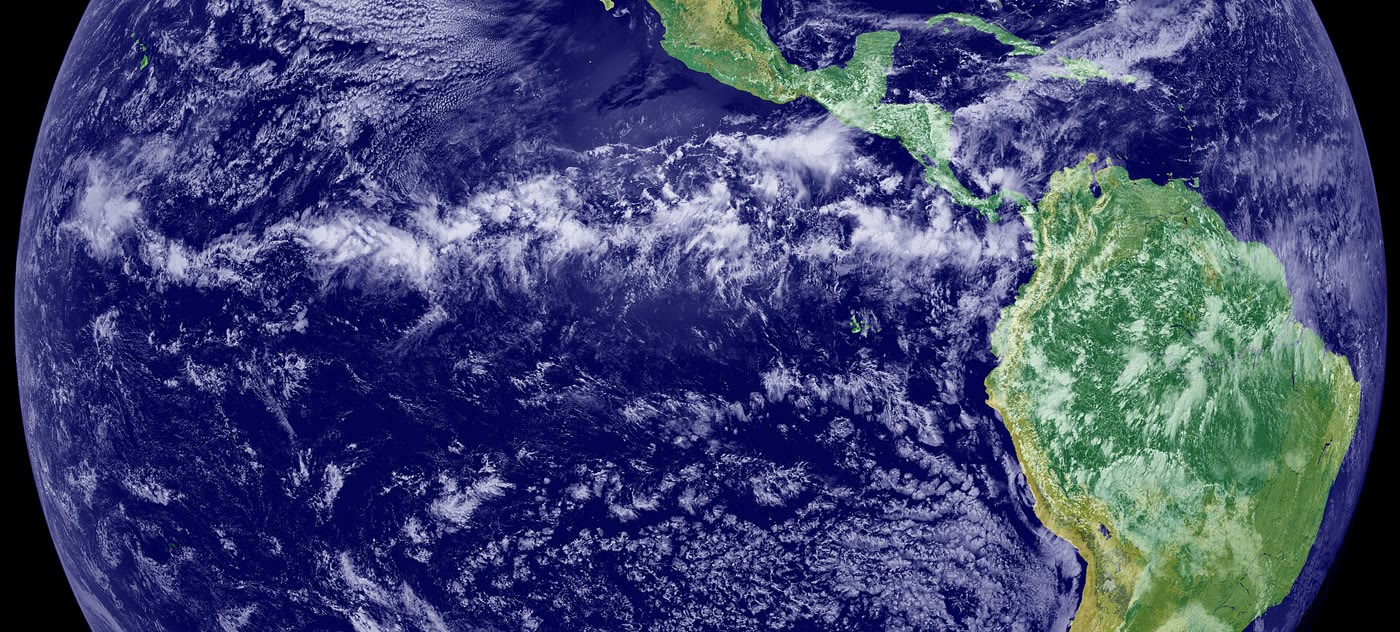
\includegraphics[width=0.8\linewidth]{images/book3/b1-itcz-goes.jpg}

{\small \omterm{def:b1:atmospheric-circulation:itcz}{Zona konvergensi intertropis} di atas Pasifik timur: sebuah garis awan terang yang melintasi laut di utara khatulistiwa, dengan Amerika Tengah dan Selatan di kanan. Citra ini menggabungkan data awan dari satelit geostasioner GOES-11 dengan warna penutup lahan. (NASA Earth Observatory, domain publik, melalui Wikimedia Commons.)}
\label{fig:b1:atmospheric-circulation:itcz-photo}
\end{omfigure}
% ledger: commons:itcz-goes

Udara yang berkonvergensi harus naik, dan udara lembap yang naik membangun awan: ITCZ adalah sabuk paling hujan di planet, dan posisinya ditelusuri oleh \omterm{def:b1:spherical-astronomy:geographic}{lintang} tempat presipitasi rerata zonal mencapai puncak. ITCZ mengikuti Matahari, dengan jeda. Dalam reanalisis puncaknya bergerak dari \ang{12.8} LS pada Februari ke \ang{10.9} LU pada September; rerata atas dua belas bulan ia berada pada \ang{2.6} LU. Rerata zonal menyembunyikan perbedaan besar antarbujur: di atas Pasifik timur dalam foto, pita berada di utara khatulistiwa, dan rerata zonal merata-ratakan pita seperti itu dengan yang berayun lebih jauh mengikuti musim.
% ledger: data:b3-ncep (computed in figdata/bachelor-1/general_circulation.py)

\begin{omfigure}
\begin{tikzpicture}
\begin{axis}[omrecord, width=0.7\linewidth, height=5.2cm, xmin=0.5, xmax=12.5, ymin=-16, ymax=16,
  xlabel={bulan}, ylabel={lintang (\unit{\degree})}, xtick={1,...,12},
  xticklabels={J,F,M,A,M,J,J,A,S,O,N,D}, ytick={-15,-10,...,15}]
% figdata/bachelor-1/general_circulation.py; ledger: data:b3-ncep
\addplot[black!40, domain=0.5:12.5] {0};
\addplot[omThm, line width=1.1pt, mark=*, mark size=1.6pt] table[x=month, y=lat] {figdata/out/bachelor-1-general_circulation-itcz.dat};
\end{axis}
\end{tikzpicture}

{\small \omterm{def:b1:spherical-astronomy:geographic}{Lintang} maksimum presipitasi rerata zonal, bulan demi bulan, antara \ang{20} LS dan \ang{20} LU: \omterm{def:b1:atmospheric-circulation:itcz}{zona konvergensi intertropis} bermigrasi ke utara pada musim panas belahan utara dan ke selatan pada musim panas belahan selatan, dua atau tiga bulan di belakang Matahari. NCEP-NCAR Reanalysis~1, rerata 1991--2020, data disediakan oleh NOAA PSL.}
\label{fig:b1:atmospheric-circulation:itcz}
\end{omfigure}
% ledger: data:b3-ncep

Di sepanjang khatulistiwa itu sendiri, tempat $f = 0$, udara bergerak lurus menuruni gradien tekanan, dan sirkulasi timur-barat muncul di atas Pasifik.

\begin{definition}[Sirkulasi Walker]\label{def:b1:atmospheric-circulation:walker}
\emph{Sirkulasi Walker}\index{sirkulasi Walker} adalah sel pembalikan timur--barat atmosfer di sepanjang Pasifik khatulistiwa: udara naik di atas air hangat di barat, di atas Benua Maritim, mengalir ke timur di ketinggian, turun di atas Pasifik timur dan kembali ke barat dekat permukaan bersama \omterm{def:b1:atmospheric-circulation:winds}{angin pasat}.
\end{definition}
% ledger: climategov:walker

\begin{omfigure}
\begin{tikzpicture}[>={Stealth[length=2mm]}, font=\scriptsize]
  \fill[blue!12] (0,0) rectangle (11,0.45);
  \shade[left color=orange!45, right color=blue!12] (0,0) rectangle (6,0.45);
  \fill[brown!45] (-0.9,0) rectangle (0,0.6);
  \fill[brown!45] (11,0) rectangle (11.9,0.6);
  \node[anchor=north] at (-0.45,-0.05) {Benua};
  \node[anchor=north] at (-0.45,-0.35) {Maritim};
  \node[anchor=north] at (11.45,-0.05) {Amerika};
  \node[anchor=north] at (11.45,-0.35) {Selatan};
  \node[anchor=north] at (5.5,-0.05) {Samudra Pasifik khatulistiwa};
  \node at (1.6,0.22) {air hangat};
  \foreach \x in {0.6,1.2,1.8} \fill[black!20] (\x,2.6) circle (0.45);
  \foreach \x in {0.9,1.5} \fill[black!25] (\x,3.0) circle (0.4);
  \draw[line width=1.2pt, omThm, ->] (9.5,0.8) -- (2.0,0.8);
  \draw[line width=1.2pt, omThm, ->] (1.2,1.0) -- (1.2,3.0);
  \draw[line width=1.2pt, omThm, ->] (2.0,3.3) -- (9.5,3.3);
  \draw[line width=1.2pt, omThm, ->] (10.3,3.0) -- (10.3,1.0);
  \node[anchor=south] at (5.75,0.85) {angin pasat, timur ke barat};
  \node[anchor=south] at (5.75,3.35) {aliran balik di atas, barat ke timur};
  \node[anchor=west, align=left] at (1.6,1.8) {udara naik,\\hujan lebat};
  \node[anchor=east, align=right] at (10.0,1.8) {udara turun,\\kering};
\end{tikzpicture}

{\small \omterm{def:b1:atmospheric-circulation:walker}{Sirkulasi Walker} di sepanjang Pasifik khatulistiwa (skematik; tinggi tidak sesuai skala): naik di barat yang hangat, mengalir ke timur di ketinggian, turun di timur dan kembali ke barat bersama \omterm{def:b1:atmospheric-circulation:winds}{angin pasat} dekat permukaan.}
\label{fig:b1:atmospheric-circulation:walker}
\end{omfigure}
% ledger: climategov:walker

\omterm{def:b1:atmospheric-circulation:walker}{Sirkulasi Walker} tidak mantap. Ketika ia melemah, gerak naik di atas Benua Maritim melemah dan udara di sana bahkan mungkin turun; ketika ia menguat, naik dan hujan di barat bertambah. Ayunan ini, El~Niño dan La~Niña, serta pembalikan musiman monsun, merupakan pokok bahasan volume Tahun~2. Selama beberapa dekade sejak 1980, penilaian IPCC 2021 menemukan penguatan \omterm{def:b1:atmospheric-circulation:walker}{sirkulasi Walker} yang \emph{sangat mungkin}, menyerupai keadaan La~Niña, dan pergeseran ke barat, dengan \emph{keyakinan sedang} pada besarnya perubahan itu.
% ledger: climategov:walker, ipcc:hadley-widening

\section{Arus jet}\label{sec:b1:atmospheric-circulation:jets}

\begin{definition}[Arus jet; arus jet subtropik dan front kutub]\label{def:b1:atmospheric-circulation:jet}
Sebuah \emph{arus jet}\index{arus jet} adalah pita sempit angin kuat, biasanya angin horizontal tinggi di troposfer, yang posisinya berubah dari hari ke hari. \emph{Arus jet subtropik}\index{arus jet subtropik} berhembus dari barat dekat tepi kutub \omterm{def:b1:atmospheric-circulation:cells}{sel Hadley}, biasanya antara \ang{20} dan \ang{30} \omterm{def:b1:spherical-astronomy:geographic}{lintang} pada ketinggian \qtyrange{12}{14}{km}. \emph{Arus jet front kutub}\index{arus jet front kutub} berhembus dari barat di atas batas antara udara kutub dan udara subtropik, antara sekitar \ang{50} dan \ang{60}; ia adalah inti cepat \omterm{def:b1:atmospheric-circulation:winds}{angin barat}, dikemudikan oleh dan mengemudikan depresi dan \omterm{def:b1:atmospheric-circulation:cyclone}{antisiklon} \omterm{def:b1:spherical-astronomy:geographic}{lintang} menengah.
\end{definition}
% ledger: nws:jets, noaajs:jet

\omterm{def:b1:atmospheric-circulation:jet}{Arus jet} biasanya ditemukan sekitar \qty{9}{km}, dapat mencapai lebih dari \qty{440}{km/h}, dan paling kuat di musim dingin setiap belahan, saat kontras suhu antara tropik dan kutub paling besar. \omterm{def:b1:atmospheric-circulation:jet}{Arus jet subtropik} adalah angin momentum sudut dari \cref{prop:b1:atmospheric-circulation:angular-momentum}, yang dijinakkan oleh pusaran; ia berada di tepi \omterm{def:b1:atmospheric-circulation:cells}{sel Hadley}, dekat \ang{30} dalam rerata musim dingin. \omterm{def:b1:atmospheric-circulation:jet}{Arus jet front kutub} mengembara ke utara dan selatan bersama depresi yang lewat, dan rerata atas globe meratakannya: dalam rerata zonal musim panas belahan utara hanya tersisa maksimum lemah \qty{21.6}{m/s} dekat \ang{42.5} LU, dan pada musim panas belahan selatan \qty{29.9}{m/s} dekat \ang{47.5} LS. Mengapa angin bertambah dengan ketinggian di mana pun suhu turun ke arah kutub, yaitu angin termal, ditunjukkan dalam volume Tahun~3.
% ledger: noaajs:jet, nws:jets, data:b3-ncep-circ (computed in figdata/bachelor-1/general_circulation.py)

\section{Latihan}

\begin{exercise}[$\star$]\label{exo:b1:atmospheric-circulation:1}
Ambil $\Omega = \qty{7.292e-5}{rad.s^{-1}}$. (a)~Hitung \omterm{def:b1:atmospheric-circulation:coriolis-parameter}{parameter Coriolis} pada \ang{0}, \ang{30}, \ang{45} dan \ang{90} LU. (b)~Hitung percepatan Coriolis horizontal angin \qty{10}{m/s} pada \ang{45} LU dan bandingkan dengan $g =
\qty{9.81}{m.s^{-2}}$. (c)~Ke arah mana ia menunjuk bila angin berhembus ke utara?
% ledger: earth:Trot
\end{exercise}

\begin{exercise}[$\star$]\label{exo:b1:atmospheric-circulation:2}
Dua isobar yang berjarak \qty{4}{hPa} berjarak \qty{400}{km} di permukaan laut, tempat $\rho =
\qty{1.225}{kg.m^{-3}}$. (a)~Hitung percepatan akibat \omterm{def:b1:atmospheric-circulation:pgf}{gaya gradien tekanan}. (b)~Bila tidak ada lain yang bekerja, berapa lama waktu yang dibutuhkan untuk mempercepat udara diam hingga \qty{10}{m/s}? (c)~Bandingkan percepatan ini dengan percepatan Coriolis angin \qty{10}{m/s} pada \ang{45} LU, dan katakan apa yang disarankan ini.
% ledger: ussa76:sea-level, earth:Trot
\end{exercise}

\begin{exercise}[$\star$]\label{exo:b1:atmospheric-circulation:3}
Pada \ang{40} LU, isobar yang berjarak \qty{4}{hPa} berjarak \qty{250}{km}; ambil $\rho =
\qty{1.225}{kg.m^{-3}}$. (a)~Hitung \omterm{def:b1:atmospheric-circulation:geostrophic}{angin geostrofik} dalam \unit{m/s} dan dalam knot
(\qty{1}{kn} = \qty{0.5144}{m/s}). (b)~Tekanan rendah berada di selatan. Dari arah mana angin
berhembus? (c)~Jelaskan panah angin (tangkai dan bulu) yang akan digambar seorang peramal cuaca.
% ledger: ussa76:sea-level, earth:Trot
\end{exercise}

\begin{exercise}[$\star$]\label{exo:b1:atmospheric-circulation:4}
Rerata tahunan reanalisis memberi, dekat tanah, angin zonal ke timur
\qty{-3.5}{m/s} pada \ang{15} LU, \qty{-4.4}{m/s} pada \ang{15} LS, \qty{+1.9}{m/s} pada
\ang{45} LU dan \qty{+6.5}{m/s} pada \ang{45} LS, dan tekanan permukaan laut
\qty{1011.8}{hPa} pada \ang{15} LU, \qty{1016.8}{hPa} pada \ang{30} LU dan
\qty{1015.8}{hPa} pada \ang{45} LU. (a)~Sebutkan sabuk angin pada setiap keempat \omterm{def:b1:spherical-astronomy:geographic}{lintang}.
(b)~Jelaskan tanda setiap angin dengan cabang permukaan sebuah sel. (c)~Di mana \omterm{def:b1:atmospheric-circulation:cells}{tekanan
tinggi subtropik} Belahan Utara menurut tekanan-tekanan ini?
% ledger: data:b3-ncep-circ
\end{exercise}

\begin{exercise}[$\star\star$]\label{exo:b1:atmospheric-circulation:5}
Gradien tekanan \qty{2}{hPa} per \qty{500}{km}, dengan $\rho =
\qty{1.225}{kg.m^{-3}}$, ditemukan pada \ang{60}, \ang{50}, \ang{30}, \ang{20},
\ang{10} dan \ang{5} LU. (a)~Hitung \omterm{def:b1:atmospheric-circulation:geostrophic}{angin geostrofik} pada setiap \omterm{def:b1:spherical-astronomy:geographic}{lintang}.
(b)~Angin sungguhan di tropik dalam jarang melebihi beberapa meter per detik di atas gradien
seperti itu. Jelaskan mengapa \omterm{def:b1:atmospheric-circulation:geostrophic}{keseimbangan geostrofik} gagal dekat khatulistiwa, dengan menggunakan
waktu $1/f$ yang dibutuhkan gaya Coriolis untuk membelokkan angin.
% ledger: ussa76:sea-level, earth:Trot
\end{exercise}

\begin{exercise}[$\star\star$]\label{exo:b1:atmospheric-circulation:6}
(a)~Dengan \cref{prop:b1:atmospheric-circulation:angular-momentum}, hitung angin dari sebuah
cincin udara yang meninggalkan khatulistiwa dalam keadaan diam, pada \ang{10}, \ang{15}, \ang{20} dan
\ang{30}; ambil $\Omega a_\oplus = \qty{464.6}{m/s}$. (b)~Hal yang sama untuk cincin yang
mulai diam pada \ang{10}, \ang{15}, \ang{20} dan \ang{30}. (c)~Cabang naik \omterm{def:b1:atmospheric-circulation:cells}{sel Hadley} tersebar
di atas \omterm{def:b1:spherical-astronomy:geographic}{lintang} alih-alih ditempatkan tepat di khatulistiwa. Bagaimana ini mengubah \omterm{def:b1:atmospheric-circulation:jet}{arus jet} yang diprediksi?
% ledger: earth:Trot, earth:Rmean
\end{exercise}

\begin{exercise}[$\star\star$]\label{exo:b1:atmospheric-circulation:7}
(a)~Sebuah kapal di Belahan Utara memiliki angin dari barat daya. Dengan hukum Buys Ballot, di mana pusat tekanan rendah? (b)~Sebuah kapal di Belahan Selatan memiliki angin dari barat laut. Di mana rendahnya?
(c)~Dekat tanah angin melintasi isobar menuju tekanan rendah. Apakah ini mengubah jawaban Anda untuk (a) dengan memutar arah rendah searah atau berlawanan arah jarum jam?
% ledger: skybrary:buys-ballot
\end{exercise}

\begin{exercise}[$\star\star$]\label{exo:b1:atmospheric-circulation:8}
(a)~Hitung massa udara antara khatulistiwa dan \ang{30} LU dan antara aras tekanan
\qty{1000}{hPa} dan \qty{100}{hPa}, dengan $a_\oplus = \qty{6371}{km}$
dan $g = \qty{9.81}{m.s^{-2}}$. (b)~Dalam rerata tahunan \omterm{def:b1:atmospheric-circulation:cells}{sel Hadley} utara reanalisis
membawa \qty{8.7e10}{kg/s}. Berapa lama waktu yang dibutuhkan untuk melewatkan massa itu
melalui sel sekali? (c)~Pertanyaan yang sama untuk sel musim dingin belahan utara,
\qty{21.4e10}{kg/s}.
% ledger: earth:Rmean, data:b3-ncep-circ
\end{exercise}

\begin{exercise}[$\star\star$]\label{exo:b1:atmospheric-circulation:9}
Anggaplah bahwa di bawah \omterm{def:b1:atmospheric-circulation:cells}{tekanan tinggi subtropik} udara turun dengan \qty{1}{cm/s}, dan bahwa udara itu tidak jenuh. (a)~Seberapa jauh ia turun dalam sehari? (b)~Seberapa banyak ia menghangat dalam sehari, bila tidak ada yang lain bekerja, dengan laju lapse adiabatik kering \qty{9.8}{K/km}? (c)~Udara tidak menghangat sebanyak itu hari demi hari. Proses mana dari \cref{ch:b1:radiation-heat-transport} yang menyeimbangkan pemanasan itu? (d)~Mengapa banyak gurun panas besar ditemukan di bawah tekanan tinggi ini?
% ledger: nws:dalr
\end{exercise}

\begin{exercise}[$\star\star\star$]\label{exo:b1:atmospheric-circulation:10}
Pada \ang{50} LU, ambil $f = \qty{1.117e-4}{s^{-1}}$ dan isobar melingkar berjari-jari
$r = \qty{500}{km}$ (\cref{rem:b1:atmospheric-circulation:gradient}). (a)~Di sekitar rendah tempat \omterm{def:b1:atmospheric-circulation:geostrophic}{angin geostrofik}
akan \qty{15}{m/s}, selesaikan $V^2/r + fV =
f|\vec v_g|$ untuk angin gradien $V$. (b)~Di sekitar tinggi, tunjukkan bahwa $V^2/r - fV + f
|\vec v_g| = 0$ hanya memiliki solusi bila $|\vec v_g| \leq fr/4$, dan hitung batas itu.
(c)~Apa yang diimplikasikan (b) untuk jarak isobar dekat pusat \omterm{def:b1:atmospheric-circulation:cyclone}{antisiklon}, dibandingkan dengan depresi?
\end{exercise}

\begin{exercise}[$\star\star\star$]\label{exo:b1:atmospheric-circulation:11}
(a)~Tunjukkan bahwa untuk $\varphi$ kecil (dalam radian) angin sebuah cincin yang meninggalkan
khatulistiwa dalam keadaan diam adalah $u \approx \Omega a_\oplus\varphi^2$. (b)~Bandingkan hampiran itu
dengan rumus eksak pada \ang{10}, dengan $\Omega a_\oplus = \qty{464.6}{m/s}$. (c)~Angin rerata
tahunan reanalisis pada \qty{200}{hPa} mencapai puncaknya \qty{27.0}{m/s} dekat
\ang{35} LU. Pada \omterm{def:b1:spherical-astronomy:geographic}{lintang} berapa cincin itu akan mencapai kelajuan ini? (d)~Apa yang dikatakan
jawaban itu tentang seberapa jauh argumen momentum sudut dapat dipercaya?
% ledger: earth:Trot, earth:Rmean, data:b3-ncep-circ
\end{exercise}

\begin{exercise}[$\star\star\star$]\label{exo:b1:atmospheric-circulation:12}
Presipitasi rerata zonal reanalisis mencapai puncaknya pada \omterm{def:b1:spherical-astronomy:geographic}{lintang} berikut, dari Januari
hingga Desember: \ang{-10.5}, \ang{-12.8}, \ang{-5.8}, \ang{-4.6}, \ang{5.5},
\ang{7.3}, \ang{8.6}, \ang{10.4}, \ang{10.9}, \ang{9.1}, \ang{7.4}, \ang{6.2}
(negatif: selatan). (a)~Hitung rerata tahunan dan rentangnya. (b)~\omterm{def:b1:spherical-astronomy:geographic}{Lintang} subsolar
mencapai ekstrem pada Juni dan Desember. Dengan berapa bulan ITCZ tertinggal di
belakangnya, dan apa dalam sistem iklim yang dapat menyimpan panas sehingga menyebabkan jeda seperti itu?
(c)~Misalkan bahwa di atas satu samudra ITCZ tetap berada di utara khatulistiwa sepanjang tahun.
Jelaskan bagaimana rerata zonal tetap dapat melintasi khatulistiwa.
% ledger: data:b3-ncep
\end{exercise}

\section{Masalah: membaca peta cuaca lintang menengah}

\begin{problem}[{Soal akhir pekan --- angin di stasiun dekat \ang{50} LU}]
\label{pb:b1:atmospheric-circulation:1}
% nilai: calc/ch28.py (peta fiktif; arus jet dari data:b3-ncep-circ)
Sebuah peta cuaca Atlantik Utara menunjukkan, dekat stasiun P pada \ang{50} LU, isobar lurus
yang berjalan dari barat ke timur, setiap \qty{4}{hPa}, dengan tekanan yang lebih rendah di utara.
P berada di antara isobar \qty{1004}{hPa} dan \qty{1008}{hPa}, yang berjarak
\qty{250}{km} di sana; tekanan permukaan lautnya \qty{1006}{hPa} dan suhu udaranya
\qty{10}{\degreeCelsius}. Peta ini fiktif, tetapi angkanya khas.
Gunakan $\Omega = 2\pi/(\qty{23.9345}{h})$, $a_\oplus = \qty{6371}{km}$, $R_d =
\qty{287.05}{J.kg^{-1}.K^{-1}}$ untuk udara kering, \qty{1}{kn} = \qty{0.514444}{m/s}.

\medskip
\noindent\textbf{Bagian I --- Gradien tekanan dan angin geostrofik.}
\begin{enumerate}
  \item Hitung massa jenis udara di P dengan hukum gas ideal.
  \item Hitung gradien tekanan horizontal di P, dalam \unit{Pa.m^{-1}}.
  \item Hitung percepatan akibat \omterm{def:b1:atmospheric-circulation:pgf}{gaya gradien tekanan}.
  \item Hitung $\Omega$ dan \omterm{def:b1:atmospheric-circulation:coriolis-parameter}{parameter Coriolis} pada \ang{50} LU.
  \item Hitung kelajuan \omterm{def:b1:atmospheric-circulation:geostrophic}{angin geostrofik} di P.
  \item Nyatakan dalam knot dan dalam \unit{km/h}.
  \item Tunjukkan bahwa waktu yang dibutuhkan \omterm{def:b1:atmospheric-circulation:pgf}{gaya gradien tekanan} saja untuk membawa
        udara diam ke kelajuan geostrofik adalah $1/f$, dan hitung, bersama dengan
        waktu $2\pi/f$ yang dibutuhkan gaya Coriolis untuk memutar angin satu lingkaran penuh.
\end{enumerate}

\medskip
\noindent\textbf{Bagian II --- Arah dan belahan.}
\begin{enumerate}[resume]
  \item Ke arah mana \omterm{def:b1:atmospheric-circulation:pgf}{gaya gradien tekanan} menunjuk di P? Ke arah mana \omterm{def:b1:atmospheric-circulation:geostrophic}{angin
        geostrofik} berhembus, dan dari \omterm{def:b1:spherical-astronomy:horizontal}{azimut} mana ia datang?
  \item Periksa jawaban Anda dengan hukum Buys Ballot.
  \item Jelaskan panah angin yang digambar di P: arah tangkai, jumlah bulu,
        dan sisi tempat mereka berdiri.
  \item Anggaplah isobar yang sama, dengan tekanan rendah di utara, ditemukan di
        \ang{50} LS. Dari arah mana angin akan berhembus?
  \item Dengan massa jenis dan gradien tekanan yang sama, hitung \omterm{def:b1:atmospheric-circulation:geostrophic}{angin geostrofik}
        pada \ang{30} LU dan \ang{60} LU.
  \item Hitung pada \ang{5} LU. Apakah hasilnya masuk akal? Jelaskan.
\end{enumerate}

\medskip
\noindent\textbf{Bagian III --- Angin di permukaan.} Sebuah anemometer di P mengukur angin
sebesar \qty{9.0}{m/s} yang melintasi isobar pada \ang{25} menuju tekanan rendah.
\begin{enumerate}[resume]
  \item Hitung rasio angin yang diamati terhadap \omterm{def:b1:atmospheric-circulation:geostrophic}{angin geostrofik}, dan komponen
        angin yang diamati sepanjang dan melintasi isobar.
  \item Dari \omterm{def:b1:spherical-astronomy:horizontal}{azimut} mana angin yang diamati berhembus?
  \item Dalam model gesekan linear \cref{prop:b1:atmospheric-circulation:friction},
        konstanta waktu $\tau$ apa yang memberi sudut yang diamati, dan kelajuan apa
        yang diprediksi model kemudian? Bandingkan dengan pengamatan.
  \item Di sekitar depresi berjari-jari \qty{500}{km}, anggaplah bahwa udara di
        kilometer terbawah mengalir ke dalam di mana-mana dengan komponen melintasi isobar
        dari soal~14 dan massa jenis dari soal~1. Hitung massa udara yang masuk ke
        depresi per detik.
  \item Udara ini harus keluar melalui puncak lapisan. Hitung kecepatan naik rerata
        di sana, dalam \unit{m/s} dan dalam meter per hari.
  \item Pada laju lapse adiabatik kering \qty{9.8}{K/km}, berapa banyak udara yang naik
        mendingin dalam sehari? Cuaca apa yang mengikutinya, dan apa yang akan terjadi
        di bawah \omterm{def:b1:atmospheric-circulation:cyclone}{antisiklon} sebagai gantinya?
\end{enumerate}

\medskip
\noindent\textbf{Bagian IV --- Arus jet di atasnya.} Angin rerata zonal pada \qty{200}{hPa} pada musim dingin belahan utara mencapai puncaknya \qty{42.3}{m/s} dekat \ang{30} LU (rerata reanalisis 1991--2020).
\begin{enumerate}[resume]
  \item Hitung kelajuan timur tanah di khatulistiwa dan di \ang{30} LU.
  \item Sebuah cincin udara meninggalkan khatulistiwa dalam keadaan diam di ketinggian dan
        mempertahankan momentum sudutnya. Hitung anginnya pada \ang{20} LU dan \ang{30} LU.
  \item Pertanyaan yang sama pada \ang{30} LU untuk cincin yang mulai diam pada \ang{10} LU.
  \item Dengan faktor berapa cincin pada soal~21 melampaui \omterm{def:b1:atmospheric-circulation:jet}{arus jet} yang
        diamati pada \ang{30} LU? Berikan dua alasan mengapa \omterm{def:b1:atmospheric-circulation:jet}{arus jet} sungguhan lebih lambat.
  \item Hitung rasio momentum sudut mutlak per satuan massa \omterm{def:b1:atmospheric-circulation:jet}{arus jet} yang diamati
        pada \ang{30} LU terhadap udara diam di khatulistiwa. Berapa bagian yang telah
        hilang di sepanjang jalan?
  \item Berapa kelajuan \omterm{def:b1:atmospheric-circulation:geostrophic}{angin geostrofik} di P, dalam meter per detik, dan bagaimana
        angin yang diukur di permukaan dibandingkan dengan itu?
\end{enumerate}
\end{problem}
